\section{本章小结}
\label{sec:newton-summary}

Newton法把优化问题变成一串线性方程：在当前点用二次模型代替目标，解$\bm{H}^{(t)}\bm{d}^{(t)}=-\bm{g}^{(t)}$，走到模型的极小点。Hessian正定时这个方向下降；解处非退化、Hessian Lipschitz且初始点足够近时，收敛是二次的。

完整的Newton步在其余情形下都可能出问题。本章把困难分成三类，每一类用一个独立的量来控制，如图~\ref{fig:newton-three-controls}所示。

\begin{BookInlineFigure}
  \centering
  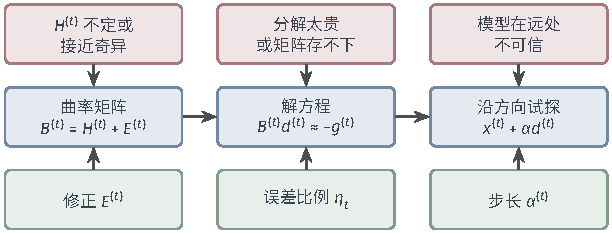
\includegraphics[width=104mm]{figures/05-optimization/02-smooth-optimization/tikz/newton-three-controls/figure.pdf}
  \caption{本章三种手段的分工。上行是遇到的困难，中行是迭代中受影响的环节，下行是对应的控制量。三个控制量互相独立，可以单独使用，也可以组合。}
  \label{fig:newton-three-controls}
\end{BookInlineFigure}

阻尼不改方向，只选步长$\alpha^{(t)}\leq1$，靠原目标的下降检验保证进展。强凸时全局线性收敛，梯度足够小后完整步自动恢复，局部二次收敛得以保留。

修正改变曲率矩阵，用$\bm{H}^{(t)}+\bm{E}^{(t)}$代替Hessian。对角平移、谱修正和修正Cholesky分解在修正量和计算量之间取舍。修正量一致有界时梯度趋于零，极限点可能是鞍点；修正消失后恢复Newton的局部行为。

非精确求解放宽线性方程，用残差比例$\eta_t$规定内层精度。比例保持小于$1$得到线性收敛，趋于零得到超线性收敛，与梯度同阶得到二次收敛。Newton-CG只用Hessian向量积，遇到非正曲率截断，方向总是下降的。

比较成本时要把外层轮数和内层工作一起计入，把远离解时的保障与解附近的速度分开看。局部收敛阶说明最后几步，总成本还取决于第一阶段的轮数和每轮的实际代价。

这些方法都要求能读取Hessian或它与向量的乘积。下一章研究不直接计算Hessian时，怎样从相邻两次梯度的变化中构造可用的曲率近似。
